\chapter{EXPERIMENTS AND VALIDATION}

\section{Experimental Scope}

The experiments in this project are written around evidence that could be verified from the repository and generated artifacts. The evaluation covers dataset construction, class-name verification, nutrition database integrity, mapping coverage, backend service behavior, frontend workflow, and qualitative detection output. The repository contains training material and deployed model metadata, but it does not contain a final metric export for the latest 72-class training run. For that reason, this report does not invent mAP, precision, or recall values. It reports the evidence that can be checked directly and leaves formal detector benchmarking as a clearly stated future evaluation step.

\begin{figure}[H]
\centering
\resizebox{0.96\textwidth}{!}{%
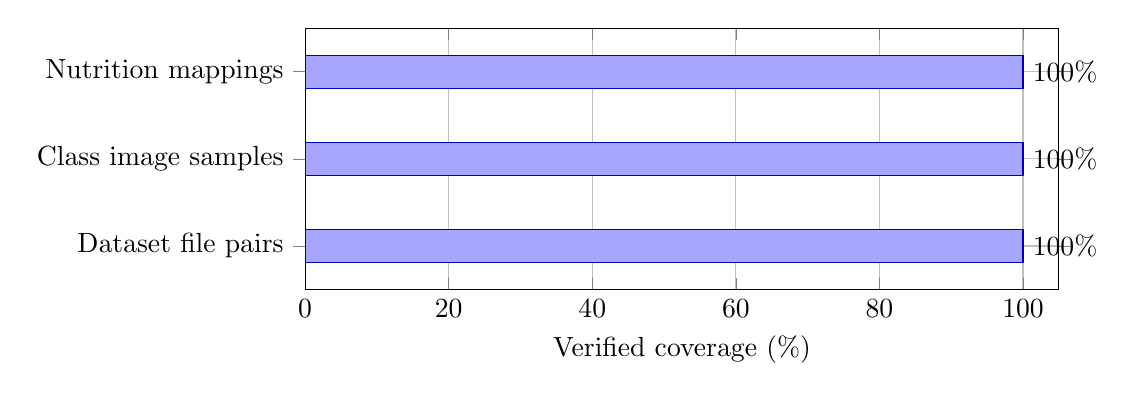
\begin{tikzpicture}
\begin{axis}[
    xbar,
    xmin=0,
    xmax=105,
    width=0.92\textwidth,
    height=4.9cm,
    xlabel={Verified coverage (\%)},
    symbolic y coords={Dataset file pairs, Class image samples, Nutrition mappings},
    ytick=data,
    nodes near coords={\pgfmathprintnumber\pgfplotspointmeta\%},
    point meta=x,
    enlarge y limits=0.25,
    grid=major,
    bar width=12pt
]
\addplot[fill=blue!35, draw=blue!70!black] coordinates {
    (100,Dataset file pairs)
    (100,Class image samples)
    (100,Nutrition mappings)
};
\end{axis}
\end{tikzpicture}
}
\caption{Verified system-level coverage used for validation}
\label{fig:validation-coverage-chart}
\end{figure}

\section{Dataset Validation}

The first validation task checks whether the merged dataset exists, contains expected split folders, and has a complete 72-class \code{data.yaml}. The generated dataset summary is shown in Table \ref{tab:generated-dataset-summary}.

\begin{table}[H]
\centering
\caption{Generated dataset summary}
\label{tab:generated-dataset-summary}
\begin{tabular}{lr}
\toprule
Property & Value\\
\midrule
Canonical classes & 72\\
Train images & 36,852\\
Train labels & 36,852\\
Validation images & 5,922\\
Validation labels & 5,922\\
Test images & 5,919\\
Test labels & 5,919\\
Total exported image-label pairs & 48,693\\
Split target ratio & 70/15/15\\
\bottomrule
\end{tabular}
\end{table}

The split counts indicate that the generated dataset is complete: every exported image has a corresponding label file. Validation and test augmentation are disabled so that held-out samples remain real images rather than transformed versions of the training data.

\section{Class Verification Experiment}

The class verification experiment generated contact sheets with four images per class. The goal was to catch practical mistakes that are easy to miss in code: class-order shifts, naming mismatches, or labels that do not match the visible food. The script found image samples for all 72 classes. Visual inspection found no class-list order problem. The issues found were sample-level annotation issues rather than class-list errors.

\begin{table}[H]
\centering
\caption{Visual class verification result}
\label{tab:visual-verification}
\begin{tabularx}{\textwidth}{L{0.35\textwidth}Y}
\toprule
Check & Result\\
\midrule
Classes checked & 72\\
Classes with image samples & 72\\
Classes without image samples & 0\\
Contact sheets generated & 8\\
Displayed samples per class & 4\\
Class-order problem found & No\\
Sample-level issues found & 3\\
\bottomrule
\end{tabularx}
\end{table}

\section{Nutrition Database Validation}

The nutrition database validation checks schema and row counts. The database contains 1,010 records in \code{indb_foods} and 103 records in \code{yolo_mappings}. The food table is based on INDB and five source-backed supplemental rows for classes that were absent from INDB. The mapping count is larger than 72 because the table includes the expanded dataset classes and legacy deployed-model labels for backward compatibility.

\begin{table}[H]
\centering
\caption{Nutrition database validation result}
\label{tab:nutrition-db-validation}
\begin{tabular}{lrr}
\toprule
Table & Purpose & Count\\
\midrule
\code{indb_foods} & INDB plus supplemental nutrition records & 1,010\\
\code{yolo_mappings} & YOLO class to database mappings & 103\\
\bottomrule
\end{tabular}
\end{table}

\section{Nutrition Mapping Coverage Experiment}

The mapping coverage experiment checks how many of the 72 dataset classes have a safe nutrition mapping. The result is shown in Table \ref{tab:mapping-coverage}.

\begin{table}[H]
\centering
\caption{Nutrition mapping coverage for 72-class dataset}
\label{tab:mapping-coverage}
\begin{tabular}{lr}
\toprule
Metric & Value\\
\midrule
Total dataset classes & 72\\
Mapped classes & 72\\
Unmapped classes & 0\\
Mapping coverage & 100.00\%\\
\bottomrule
\end{tabular}
\end{table}

The classes \code{bhakarwadi}, \code{ghevar}, \code{jalebi}, \code{khandvi}, and \code{nandu_masala} were not present as safe INDB rows, so verified supplemental entries were added with source metadata. The supplemental values use a FatSecret product nutrition label for \code{bhakarwadi} and Clearcals recipe nutrition pages for the remaining dishes \cite{fatsecret_bhakarwadi_2026,clearcals_ghevar_2026,clearcals_jalebi_2026,clearcals_khandvi_2026,clearcals_nandu_kari_2026}. This keeps the full 72-class dataset usable while avoiding unsafe fuzzy substitutions.

\begin{table}[H]
\centering
\caption{Verified supplemental nutrition rows}
\label{tab:supplemental-nutrition}
\begingroup
\small
\setlength{\tabcolsep}{3pt}
\begin{tabularx}{\textwidth}{L{0.18\textwidth}Yrrrr}
\toprule
Class & Database row & kcal & Protein & Carbs & Fat\\
\midrule
\code{bhakarwadi} & \code{Bhakarwadi} & 510.0 & 10.76 & 57.03 & 26.55\\
\code{ghevar} & \code{Ghevar} & 351.2 & 3.5 & 39.6 & 19.9\\
\code{jalebi} & \code{Jalebi} & 316.8 & 3.4 & 44.6 & 13.8\\
\code{khandvi} & \code{Khandvi} & 232.7 & 9.3 & 21.7 & 12.1\\
\code{nandu_masala} & \code{Nandu Kari (Crab masala)} & 128.1 & 7.0 & 7.0 & 8.0\\
\bottomrule
\end{tabularx}
\endgroup
\end{table}

\section{Service Lookup Validation}

Service-level lookup validation was performed for classes that previously suffered from incorrect fuzzy matches. The corrected results are shown in Table \ref{tab:lookup-validation}.

\begin{table}[H]
\centering
\caption{Corrected nutrition lookup examples}
\label{tab:lookup-validation}
\begin{tabularx}{\textwidth}{L{0.28\textwidth}Y}
\toprule
Input class & Returned INDB display name\\
\midrule
\code{aloo_gobi} & \code{Potato cauliflower (Aloo gobhi)}\\
\code{palak_paneer} & \code{Spinach paneer (Palak paneer)}\\
\code{rice} & \code{Boiled rice (Uble chawal)}\\
\code{AlooGobi} & \code{Potato cauliflower (Aloo gobhi)}\\
\code{WhiteRice} & \code{Boiled rice (Uble chawal)}\\
\bottomrule
\end{tabularx}
\end{table}

This confirms that the revised database mapping handles both canonical dataset labels and legacy deployed-model labels.

\section{Backend API Validation}

The backend validation focuses on service readiness and response structure. The analysis endpoint returns HTTP 503 if vision or nutrition services are unavailable. Empty images, non-image MIME types, and uploads exceeding 10 MB are rejected. The analysis response includes food label, confidence, bounding box, nutrition source, macro values, and food-not-found status. This structured response is important because the frontend depends on predictable fields for visualization and macro tracking.

\section{Frontend Workflow Validation}

The frontend workflow was validated qualitatively by uploading sample food images and verifying that the interface displays bounding boxes, detected labels, confidence values, nutrition cards, serving controls, and recommendation text. Figure \ref{fig:detection-overlay} in Chapter 5 shows a successful example with Bhatura and Chole detections. The interface also handles no-food responses and backend error messages.

\begin{figure}[H]
\centering
\begin{tikzpicture}[
    flowstep/.style={draw, rounded corners, align=center, minimum width=3.1cm, minimum height=0.85cm, fill=green!8},
    check/.style={draw, rounded corners, align=center, minimum width=3.1cm, minimum height=0.85cm, fill=orange!10},
    arrow/.style={-Latex, thick},
    node distance=0.75cm and 0.8cm
]
\node[flowstep] (upload) {Upload image};
\node[flowstep, right=of upload] (preview) {Preview and send};
\node[flowstep, right=of preview] (overlay) {Render boxes};
\node[check, below=of upload] (serving) {Adjust serving};
\node[check, right=of serving] (macros) {Update macros};
\node[check, right=of macros] (advice) {Show advice};
\draw[arrow] (upload) -- (preview);
\draw[arrow] (preview) -- (overlay);
\draw[arrow] (overlay) -- (advice);
\draw[arrow] (upload) -- (serving);
\draw[arrow] (serving) -- (macros);
\draw[arrow] (macros) -- (advice);
\end{tikzpicture}
\caption{Frontend workflow checks used during qualitative validation}
\label{fig:frontend-workflow-validation}
\end{figure}

\section{Macro Calculation Validation}

Macro validation checks whether a target calorie value is converted correctly to grams. For example, for a 2,000 kcal weight-loss goal with a 40/35/25 split, the carbohydrate target is 200 g, protein target is 175 g, and fat target is approximately 56 g. Health profiles modify these base splits. The formula was discussed in Chapter 3.

\section{Experimental Findings}

The experiments show that the dataset and application pipeline are internally consistent. The system can detect food classes, map all 72 expanded dataset classes to nutrition records, and display results in the frontend. The major remaining experimental gap is the lack of a complete final metrics report for the latest 72-class trained model. Future work should add a formal evaluation table including mAP@50, mAP@50:95, per-class precision, per-class recall, confusion matrix, and inference latency.
